
\documentclass[letterpaper, 10pt]{article}
\topmargin-2.0cm

\usepackage{fancyhdr}
\usepackage{hyperref}
\usepackage{lastpage}
\usepackage[dvips]{color}
\usepackage{graphicx}
\usepackage[usenames,dvipsnames,svgnames,table]{xcolor}

% Color Information from -
% http://www-h.eng.cam.ac.uk/help/tpl/textprocessing/latex_advanced/node13.html

\advance\oddsidemargin-1in
\advance\evensidemargin-1.5cm
\textheight9.2in
\textwidth6.75in
\newcommand\bb[1]{\mbox{\em #1}}
\def\baselinestretch{1.05}

\newif \ifcomments
%\commentstrue

\ifcomments
\newcommand{\jikk}[1]{{---\textcolor{red}{#1}---}}
\else
\newcommand{\jikk}[1]{}
\fi

\newcommand{\hsp}{\hspace*{\parindent}}
\definecolor{gray}{rgb}{0.4,0.4,0.4}

\begin{document}
\thispagestyle{fancy}

% Leave Left and Right Header empty.
\lhead{}
\rhead{}

\renewcommand{\headrulewidth}{0pt} 
\renewcommand{\footrulewidth}{0pt} 

\fancyfoot[C]{\footnotesize
\textcolor{gray}{http://www.cs.columbia.edu/$\sim$jikk/application}} 

\pagestyle{fancy}
\lhead{\textcolor{gray}{\it Kangkook Jee}}
\rhead{\textcolor{gray}{\thepage /\pageref{LastPage}}}

% This kind of makes 10pt to 9 pt.
\begin{small}

%\vspace*{0.1cm}
\begin{center} {\LARGE \bf TEACHING STATEMENT}\\ \vspace*{0.1cm} {\normalsize
Kangkook Jee (jikk@cs.columbia.edu)} \end{center}
% Begin with my teaching philosophy.
University education should provide chances for student to cultivate their
potentials to succeed in their future careers as a competent computer science
professionals.  
%
As an CS educator, I focus on preparing students with principled understanding
about fundamental/theoretical CS topics along with known best practices both
from academia and industry for them to learn how to create reliable and
scalable products.

%I enjoy human interactions in the course of teaching.

\subsubsection*{In class teaching experiences}

During my PhD, I taught Columbia University's COMS3103-3: Programming Language
Python\footnote{\url{http://www.cs.columbia.edu/~jikk/teaching/3101-3/index.html}}.
%
% The course begin with 22 students and 14 students completed the course.  for
% failing to set appropriate level for assignment.
%
Although it was my first university level teaching experience, I enjoyed much
from the whole process of building a course from scratch, deliver prepared
materials, and making interactions with students.
% 
The course is largely composed of two distinct phases. The first one is about
language fundamentals while the second one focuses on specific topics/modules
relevant to student's interest. Establishing the latter was especially
challenging since the class comprised undergraduates, MS and PhD students from
diverse disciplines of CS, economics, philosophy, English literature and so on.
%
I began the semester surveying to know about students' expectation and the
background and I also attempted to maximize to face-to-face interaction with
each student throughout the semester.
% 
Students were to fulfill four homework assignments and a class project to
complete the course. 
%
Assignments were designed not only to assess student's comprehension about
course materials but also to introduce primitive CS concepts to non-major
students.
%
% basic data structures such as queue and stack as well as an algorithmic
% concept of TSP were used.
%
I also realized that it requires  substantial amount of time and effort to
write a new set of assignments each time given that students always can search
for solutions for recycled problems. 
%
Regarding a class project, students were to made teams of 3 $\sim$ 4 members to
conduct to a project relevant to their research interest.
%
It was an exciting experience to find out that many of project output were so
creative and reached out beyond my expectation.
%
% Some impressive example include search engine for Columbia university, NLP
% project that establishes character network extraction analyzing novel text
% done by English literature major.
%

Compensating for a challenging task of doing a class from the beginning to the
end, the course evaluation
result\footnote{\url{http://www.cs.columbia.edu/~jikk/teaching/3101-3/evaluation.html}}
performed by student were encouraging, especially for non-naive English speaker
as I am. In a nutshell, students rated 4.45/5 for overall course quality and
4.64/5 for amount they learned from the class.

%CS as a moving target
\subsubsection*{Designing new courses} 

CS as an academic area and its many sub-fields are still young and vibrantly
evolving. Therefore, it is required to timely design and offer new courses that
reflect recent trends/changes/updates without loosing the connections to
fundamental theories supporting the topic. \jikk{improve it} From here, I will
introduce brief descriptions for a couple of new course offerings.
%

{\bf C++ and new standard~(C++11)} In the history of programming languages, C++
occupies a unique position and it enters into interesting new stage with its
recent announcement for a new standard(C++11) and concrete roadmap projecting a
decade ahead which are well appreciated by community.
%Although many complain for its syntax being too complex and its features being
%not organized and only being grossly accumulated over time.  But, there is few
%alternative when we look for the programming language that supports the
%low-level access and close-to native performance in a scalable way.
%
%Based C language, reaching out to absorb high-level language concepts
%including OOP paradigm, C++ enters interesting new stage with its recent
%announcement for a new standard(C++11) and concrete roadmap projecting a
%decade ahead which are well appreciated by community.
%
By having a course about C++ and its new standard, we can expect students not
only to pick up a language its newly added features but also to understand how
a low level language~(based on C) reaches out to implements high level paradigm
of OOP. 

{\bf Advanced compiler course: Instrumentations from source to binary} 
%What else courses I'm capable of/interested in teaching.
Throughout my research career, I explored software instrumentation techniques
from different software stacks. 
%
Stages of compiling a source code into a binary and loading it into a memory
space for execution provide instrumentation opportunities.

a source code is first translated into compiler IR to be a target for
optimizations. IR is translated into object file and linker    complied to
generate binaries.

%\begin{figure}[tb]
%	\centering
%	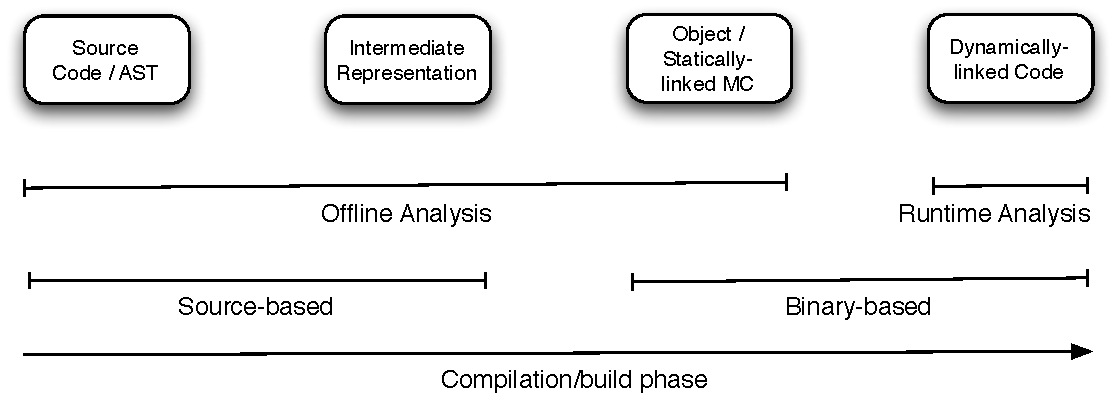
\includegraphics[width=0.5\linewidth]{figs/inst0.pdf}
%	\caption{Insturmentation}
%	\label{fig:decoupling}
%\end{figure}

%I can teach wide ranges of CS core curriculum.
%\begin{itemize}
%\item Introduction to Computer Science
%\item Programming language courses -- C, C++, Java, Python 
%\item Senior level system courses -- desktop and mobile operating system,
%  programming language.
%\item Graduate level course: advanced compiler course -- instrumentation for
%  software monitoring and protection.
%\end{itemize}
%

\subsubsection*{Summary}
here is a section for summary.
\end{small}
\end{document}

